\documentclass{homework}
%\usepackage{ctex}
\author{马成 3190102309}
\class{Num PDE}
\date{\today}
\title{Homework \#1(Chapter 8)}
%\address{Bayt El-Hikmah}

\graphicspath{{./media/}}

\begin{document} \maketitle

\question Exercise 8.8.

	In the following proof, $||\cdot||_2$ is denoted by $||\cdot||$. According to \textbf{Definition 8.4} and \textbf{Lemma 8.5}, we have
	\begin{eqnarray}\label{eq:1}
		\frac{||\textbf{e}||}{||\textbf{u}||} = \frac{||A^{-1} \textbf{r}||}{||A^{-1} \textbf{f}||}
	\end{eqnarray}
	
	Since
	\begin{eqnarray}\label{eq:2}
		A^{-1} \textbf{r} = A^{-1} \cdot \textbf{r},\quad r = A \cdot A^{-1}\textbf{r},
	\end{eqnarray}
	we have
	\begin{eqnarray}\label{eq:3}
		\frac{||\textbf{r}||}{||A||} \leq ||A^{-1}\textbf{r}|| \leq ||A^{-1} \textbf{r}||
	\end{eqnarray}
	
	Similarly,
	\begin{eqnarray}\label{eq:4}
		\frac{||\textbf{f}||}{||A||} \leq ||A^{-1}\textbf{f}|| \leq ||A^{-1} \textbf{f}||
	\end{eqnarray}
	
	Substitute \ref{eq:3} and \ref{eq:4} into \ref{eq:1}, then we have 
	\begin{equation}
		\frac{1}{\operatorname{cond}(A)} \frac{\|\mathbf{r}\|_{2}}{\|\mathbf{f}\|_{2}} \leq \frac{\|\mathbf{e}\|_{2}}{\|\mathbf{u}\|_{2}} \leq \operatorname{cond}(A) \frac{\|\mathbf{r}\|_{2}}{\|\mathbf{f}\|_{2}}
	\end{equation}

\question Exercise 8.9.

	According to \textbf{Example 8.2}, we have
	\begin{eqnarray}
		\begin{aligned}
			\cond(A) &= \frac{\max \lambda_k(A)}{\min \lambda_k(A)} = \frac{\sin^2 \frac{n-1}{2n}\pi}{\sin^2 \frac{1}{2n}\pi} \\
			&= \frac{1}{\tan^2 \frac{1}{2n} \pi } \approx \frac{4n^2}{\pi^2}
		\end{aligned}
	\end{eqnarray}

	\textbf{For $n = 8$}, we have
	\begin{eqnarray}
		\cond(A) \approx \frac{256}{\pi^2}
	\end{eqnarray}
	
	\textbf{For $n = 1024$}, we have
	\begin{eqnarray}
		\cond(A) \approx \frac{4194304}{\pi^2}
	\end{eqnarray}
	
\question Exercise 8.12.

\question Exercise 8.15.

	\begin{figure}[H]
		\centering
		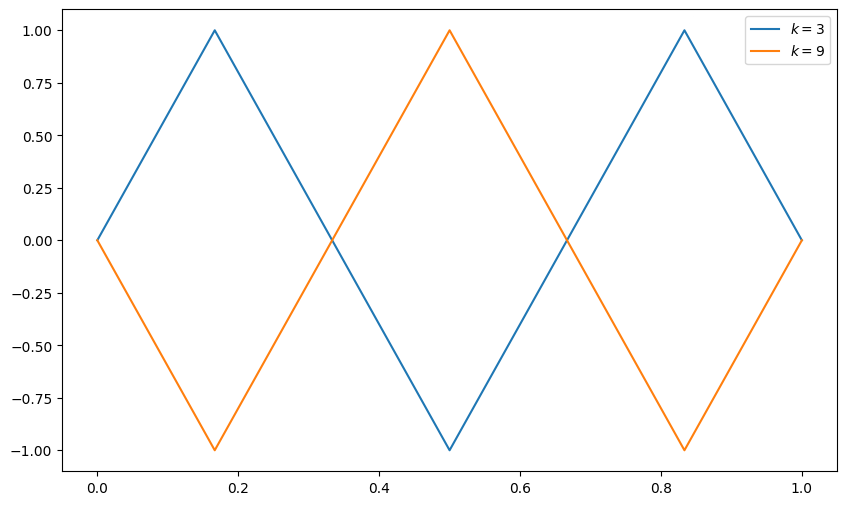
\includegraphics[width=\textwidth]{./media/Ex8_15.png}
	\end{figure}
	\lstinputlisting[language=Python, caption={code for plot}, label=gcd]{code/Ex8_15.py}

\question Exercise 8.19.
	
	According to \textbf{Definition 8.17}, we have
	\begin{eqnarray}
		\begin{aligned}
			\be^{(l+1)} &= \bu^{(l+1)} - \bu = T\bu^{(l)} + \bc - \bu \\
			&= T\bu^{(l)} + \bc - T\bu -c\\
			&= T(\bu^{(l)} - u) = T \be^{(l)}
		\end{aligned}
	\end{eqnarray}
	
	Thus $\be^{(l)} = T^l \be^{(0)}$.
	
	To prove the proposition, it suffices to show that if $A \in \CC^{n\times n}$, then
	\begin{eqnarray}
		\lim_{k\ra\infty} A^k = 0 \iff \rho(A) < 1
	\end{eqnarray}
	
	\textbf{(1)"$\Ra$"}\quad Assume $\lambda\in\lambda(A):\ \rho(A)=|\lambda|$, then $\forall k$, we have $\lambda^k \in \rho(A^k)$. So
	\begin{eqnarray}
		\begin{aligned}
			\rho(A)^k = |\lambda|^k \leq \rho(A^k) \leq ||A^k||_2,\quad \forall k
		\end{aligned}
	\end{eqnarray}
	
	Thus $\rho(A) < 1$.
	
	\textbf{(2)"$\La$"}\quad If $\rho(A) < 1$, then for any matrix norm $||\cdot||$, we have $||A|| < 1$. So
	\begin{eqnarray}
		0 \leq ||A^k|| \leq ||A||^k \ra 0,\ k \ra \infty
	\end{eqnarray}
	
	Thus $\lim_{k\ra\infty} A^k = 0$.
	
\question Exercise 8.24.

	According to \textbf{Definition 8.22}, we have
	\begin{eqnarray}
		\begin{aligned}
			\bu^{(l+1)} &= (1-\omega) \bu^{(l)} + \omega(T\bu^{(l)}+\bc) \\
			&= [(1-\omega)I + \omega T] \bu^{(l)} + \omega\bc
		\end{aligned}
	\end{eqnarray}
	
	So 
	\begin{eqnarray}
		\begin{aligned}
			T_\omega &= (1-\omega)I - \omega D^{-1}(L+U) \\
			&= I - \omega D^{-1} (L+U+D) = I - \omega D^{-1} A = I - \frac{\omega h^2}{2} A.
		\end{aligned}
	\end{eqnarray}
	
	Since 
	\begin{eqnarray}
		\begin{aligned}
			w_k T_\omega &= w_k (I - \frac{\omega h^2}{2} A)
			= w_k - \frac{\omega h^2}{2} \lambda_k(A) w_k
			= (1 - \frac{\omega h^2}{2}\lambda_k(A)) w_k, 
		\end{aligned}
	\end{eqnarray}
	so 
	\begin{eqnarray}
		\begin{aligned}
			\lambda_k(T_\omega) = 1 - \frac{\omega h^2}{2}\lambda_k(A) = 1 - 2\omega \sin^2 \frac{k\pi}{2n},
		\end{aligned}
	\end{eqnarray}
	and the eigenvector of $\lambda_k(T_\omega)$ is still $w_k$.
	
\question Exercise 8.25.
	\begin{figure}[H]\label{fig:25}
		\centering
		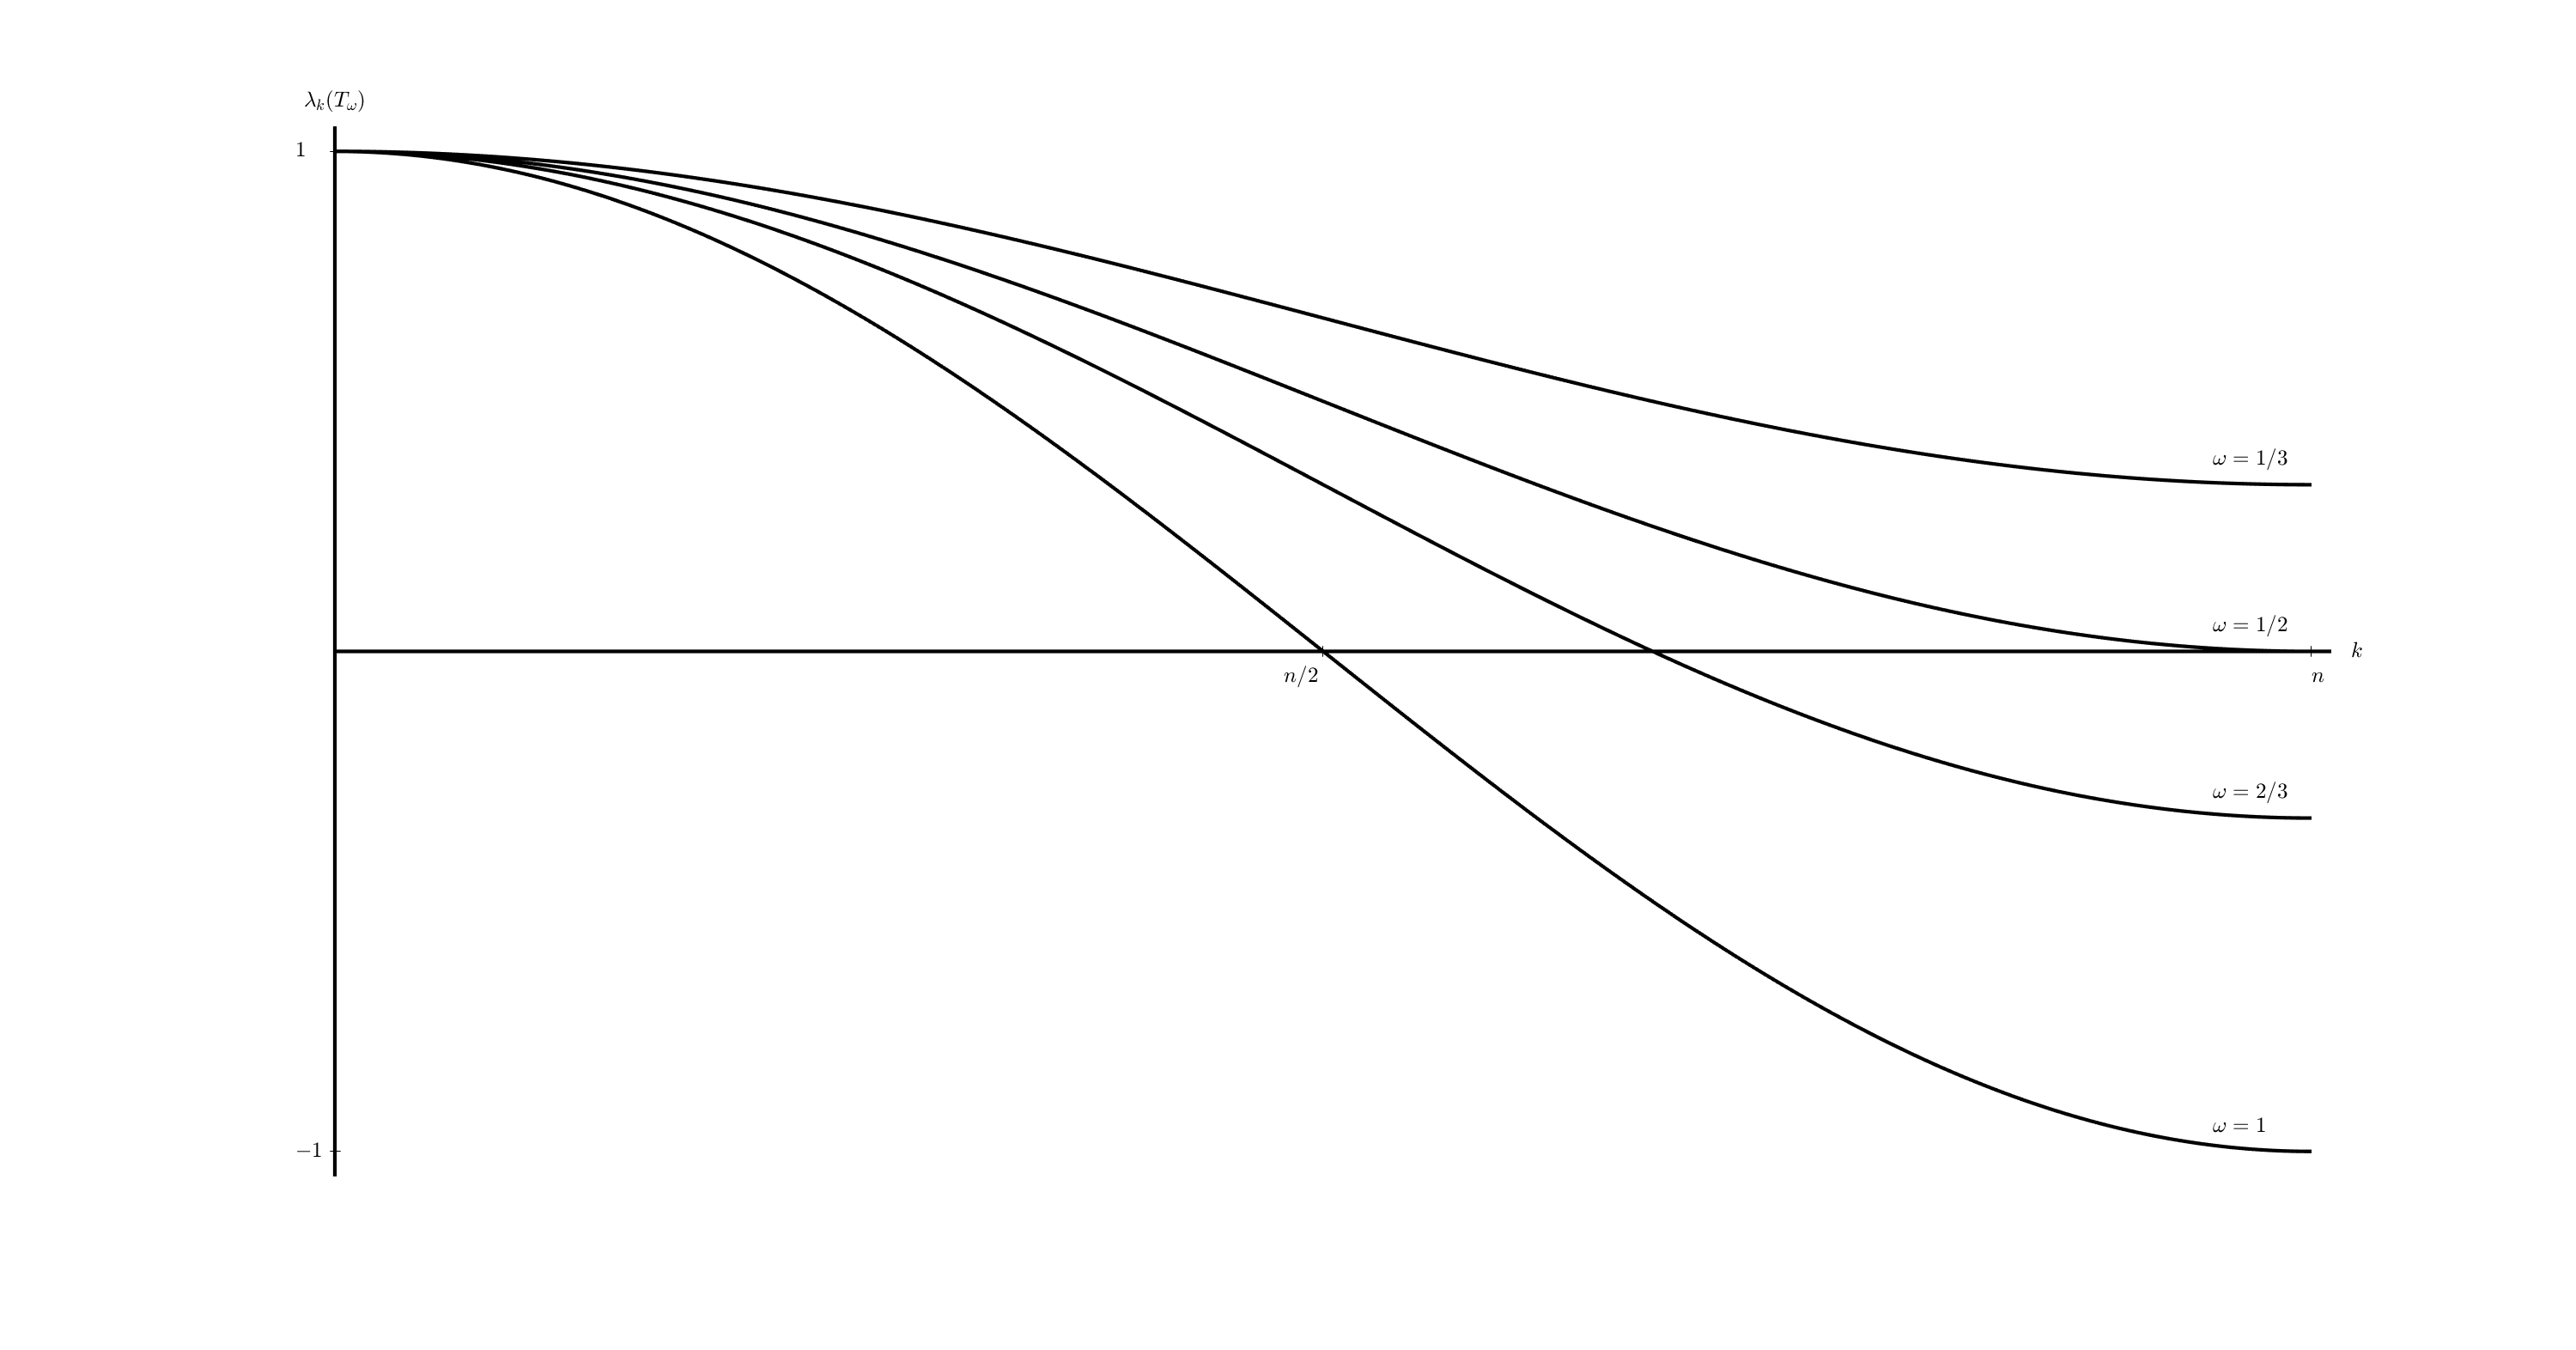
\includegraphics[width=\textwidth]{./media/Ex8_25.png}
	\end{figure}
	\lstinputlisting[language=Matlab, caption={code for the above figure}, label=gcd]{code/Ex8_25.m}
	
	Since when $n = 64$
	\begin{eqnarray}
		\begin{aligned}
			\min_{\omega\in[0,1]}\rho(T_\omega) = \min_{\omega\in[0,1]} \max_{k\in[1,n-1]} \lambda_k(T_\omega) = 1 - 2\sin^2 \frac{\pi}{128}
			= 0.9988 > 0.9986,
		\end{aligned}
	\end{eqnarray}
	then $\forall \omega\in[0,1]$ $\rho(T_\omega) \geq 0.9986$.
	
\question Exercise 8.28.

	To make the code more clear, we use Python instead.
	\begin{figure}[H]
		\begin{minipage}[t]{0.45\textwidth}
			\centering
			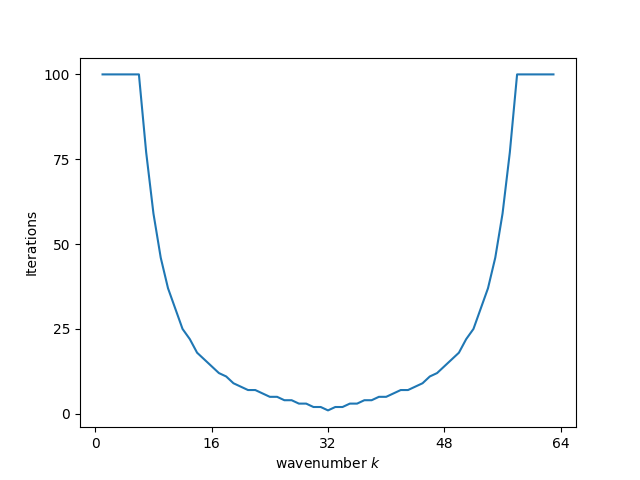
\includegraphics[scale = 0.5]{Ex8_28_a.png}
			\caption{$\omega = 1$}
		\end{minipage}
		\qquad
		\begin{minipage}[t]{0.45\textwidth}
			\centering
			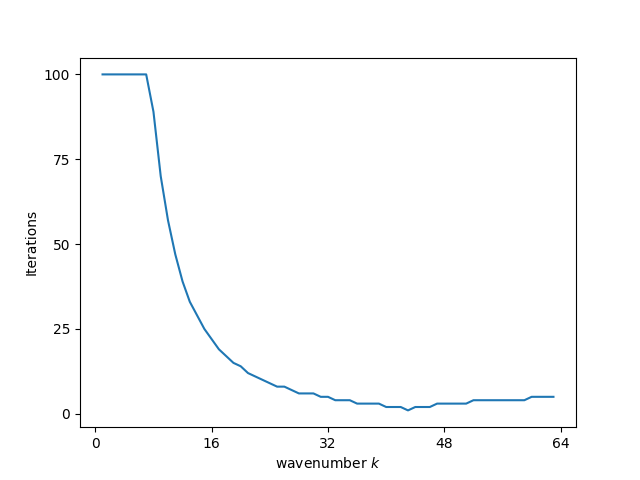
\includegraphics[scale = 0.5]{Ex8_28_b.png}
			\caption{$\omega = 2/3$}
		\end{minipage}
	\end{figure}
	\lstinputlisting[language=Python, caption={code for the above figure}, label=gcd]{code/Ex8_28.py}
	
\end{document}